% !TeX root = main.tex
\documentclass{./packages/informe}
\usepackage{./packages/caratula}
\graphicspath{./files/src/.media/}

\hyphenation{si-guien-te}
\hyphenation{ge-ne-ra-li-dad}
\hyphenation{con-si-de-ra-mos}
\hyphenation{se-cuen-cia-les}

\begin{document} 

% caratula 
\titulo{TP 1: Técnicas Algorítmicas}
\subtitulo{}
\fecha{23 de Abril, 2023}
\materia{Algoritmos y Estructuras de Datos III}
% \grupo{Grupo 18}

\integrante{Zaid, Pablo}{-}{-}
\integrante{Arienti, Federico}{316/21}{fa.arienti@gmail.com}

\maketitle


% palabras clave y resumen
\addtocontents{toc}{\protect\setcounter{tocdepth}{0}}
\section*{resumen}
\addtocontents{toc}{\protect\setcounter{tocdepth}{3}}
Una estrategia \textit{golosa} ---o \textit{greedy}--- es una estrategia de resolución de problemas, por lo general de optimización, que aprovecha las propiedades intrínsecas a una solución óptima para resolver un problema de manera correcta y computacionalmente eficiente. En relación a la estrategia de \textit{programación dinámica}, el método se basa\footnote{ Ver Thomas H. Cormen; Charles E. Leiserson; Ronald L. Rivest y Clifford Stein. Introduction to algorithms.
2009. Sección 16.2: \textit{Elements of a greedy strategy}.} en la aplicación de la propiedad de \textit{subestructura óptima}\footnote{ No todo problema tiene este propiedad y no todo problema que la posee tiene una solución \textit{greedy}.}: una solución óptima a un problema incorpora soluciones óptimas a subproblemas relacionados. Sin embargo, a diferencia de esta estrategia, los algoritmos \textit{greedy} obtienen una solución por medio de decisiones que ``\textit{contemplan la información inmediatamente disponible, sin preocuparse por los efectos que estas decisiones puedan tener en el futuro}''\footnote{ Ver Gilles Brassard y Paul Bratley. Fundamentals of Algorithmics. 1995. Capítulo 6: \textit{Greedy Algorithms}.}. Un comportamiento que requiere que el problema tenga la propiedad de \textit{selección golosa}: una solución globalmente óptima se puede obtener a partir de decisiones localmente óptimas. 

El siguiente informe evalúa la aplicación del método sobre el problema de la \textit{selección de actividades}, que se enmarca dentro del más general \textit{problema de la fiesta}. Además, evalúa la eficiencia del algoritmo resultante de manera empírica.

$\\$
\noindent Palabras clave: \textit{Algoritmos golosos, estrategias algorítmicas, selección de actividades.}

% \newpage

% contenido
\tableofcontents
\newpage

% introduccion
\section{El problema de la selección de actividades}
\vspace{1em}
El problema de la selección de actividades que consideraremos tiene la siguiente premisa. Dado un conjunto 
\begin{equation}\\\nonumber
    A := \{a_1\ ...\ a_n \}
\end{equation}
de actividades disponibles, donde, para todo $1 \leq i \leq n$, la actividad $a_i$ se representa por el intervalo $[s_i,\ t_i)$ ---que corresponde, respectivamente, al tiempo de inicio y finalización de la actividad---,  queremos encontrar un subconjunto de $A$ que nos permita realizar la mayor cantidad de actividades posibles. 

En esto, queremos elegir las actividades con la restricción que, para todo par de actividades $a_i$ y $a_j$ seleccionadas, $1 \leq i,\ j \leq n$, $a_i$ y $a_j$ no se solapen en el tiempo. Es decir, $s_i \geq t_j$ o $s_j \geq t_i$. Por ejemplo, si
\begin{equation}\\\nonumber
    A := \{[1,\ 3),\ [1,\ 4),\ [3,\ 6),\ [4,\ 7),\ [7,\ 8)\}
\end{equation}
\noindent luego las soluciones óptimas son $\{[1,\ 3),\ [3,\ 6),\ [7,\ 8)\}$ y $\{[1,\ 4),\ [4,\ 7),\ [7,\ 8)\}$. 

Como condición extra, limitaremos el tiempo de la actividad $a_i$, para todo $1 \leq i \leq n$, de manera tal que $1 \leq s_i < t_i \leq 2n$. 

%\vspace{0.5em}
\subsection{Demostración de la propiedad de subestructura óptima}

Como preámbulo a la aplicación de una estrategia \textit{golosa} para resolver el problema, veamos primero que el problema tiene la propiedad de \textit{subestructura óptima}. 

\begin{proof}[Demostración]
    Consideremos una solución óptima $S \subset A$ que contiene, sin pérdida de generalidad, a alguna actividad $a_i \in A$ para $1 \leq i \leq n$. Luego, podemos particionar tanto a $S$ como a $A$ entre aquellas actividades que terminan antes que comience $a_i$: $S_{<i}$ y $A_{<i}$; y aquellas que comienzan después de que termine $a_i$: $S_{>i}$ y $A_{>i}$. 

    Si estas particiones de $S$ no son, correspondientemente, óptimas para las particiones de $A$, entonces existe algún subconjunto de actividades $S'_{<i} \subset A_{<i}$ que tiene un tamaño mayor que la partición $S_{<i}$ que consideramos y, de igual manera, existe una solución mayor $S'_{>i}$ para el subconjunto de actividades $A_{>i}$.
    
    Sigue entonces que $S$ no es óptima, ya que podemos formar una solución mejor si consideramos $S'_{<i} \cup \{a_i\} \cup S'_{>i}$, lo que es un absurdo.
\end{proof}

Luego, estamos en condiciones de evaluar el problema como una serie de decisiones que reducen el problema a una serie de subproblemas más chicos. La siguiente demostración prueba que, además, podemos alcanzar un óptimo por medio de decisiones locales. 

%\vspace{0.5em}
\subsection{Demostración de la propiedad de selección golosa} Consideremos ahora la siguiente estrategia \textit{golosa}: elegir la actividad que finalice primero, de entre todas las actividades que sigan disponibles. Vamos a demostrar que esta estrategia es correcta.

\begin{proof}[Demostración]
    Notemos primero que, si la solución parcial $B_1\ ...\ B_i$ de actividades seleccionadas ---que brinde un algoritmo goloso que implemente esta estrategia--- se puede extender a una solución óptima, para todo $0 \leq i \leq n$, entonces la estrategia es correcta. Lo demostraremos por inducción.

    Para el caso base, $i = 0$, el algoritmo todavía no eligió ninguna actividad. Luego, podemos extender la solución a una solución óptima de manera trivial.

    Supongamos ahora, para $i > 0$, que tenemos una solución parcial $B_1\ ...\ B_i$ de actividades elegidas por nuestro algoritmo que se puede extender a una solución óptima
    \begin{align}\nonumber
        B_1\ ...\ B_i,\ C_{i+1}\ ...\ C_j
    \end{align}
    donde, sin pérdida de generalidad, vamos a suponer que la secuencia de actividades sin solapamiento $C_{i+1}\ ...\ C_j$ está ordenada por tiempo de finalización. 

    Notar que, por nuestro método de selección, $B_1\ ...\ B_i$ también debe estar ordenado de la misma manera. Luego, todas las actividades $C_{i+1}\ ...\ C_j$ deben empezar después de que termine $B_i$ para que la extensión sea válida. Si no, habría solapamientos, ya que, por definición de la estrategia, deben terminar después que $B_i$.

    Consideremos ahora la solución parcial golosa $B_1\ ...\ B_{i+1}$, donde $B_{i+1}$ es la actividad cuyo momento final ocurre antes entre todas las actividades restantes y no se solapa con las actividades ya seleccionadas. 

    Como $B_{i+1}$ debe terminar antes que $C_{i+1}$ o $B_{i+1} = C_{i+1}$, entonces $B_{i+1}$ no puede solaparse con ninguna actividad $C_{i+2}\ ...\ C_j$. Esto se debe a que $C_{i+1}$ no lo hacía y, por hipótesis inductiva, es la actividad que termina antes en la extensión. Luego, $B_1\ ...\ B_{i+1}$ se puede extender por reemplazo directo a la solución óptima 
    \begin{align}\nonumber
        B_1\ ...\ B_{i+1},\ C_{i+2}\ ...\ C_j
    \end{align}
    lo que concluye la demostración.
\end{proof}

%\vspace{1em}
\subsection{El algoritmo} En base a estas propiedades, podemos considerar el siguiente algoritmo \textit{goloso} como una resolución al problema de \textit{selección de actividades}. 

%\vspace{1em}
\lstinputlisting[mathescape=true, language=pseudo, label=actividades, caption={Pseudocódigo para la \textit{selección de actividades}.}]{files/src/.code/act.pseudo}

El mismo itera sobre las actividades en $A$ por orden de finalización. En base a la estrategia golosa, decide incluir, o no, una actividad si y sólo si comienza después de que termine la última actividad que ya incluyó, cuyo tiempo de finalización se guarda en la variable $i$. Dado que no tiene sentido considerar tiempos negativos, inicializamos $i$ en $0$.

%\vspace{1em}
\subsection{Complejidad temporal y espacial} El comportamiento del algoritmo depende del método de ordenamiento que elijamos y de las características de la estructura subyacente al conjunto $P$ (en particular, si la inserción de un elemento se puede realizar en tiempo constante). 

Respecto al método de ordenamiento, dado que los tiempos de finalización estan acotados por $2n$, podemos utilizar \textit{counting sort} para garantizar una complejidad de peor caso, tanto temporal como espacial, de orden lineal. Notar que \textit{counting sort} tiene complejidad $O(m + k)$ donde $m$ es la cantidad de elementos a ordenar y $k$ es la diferencia entre el valor máximo y mínimo en el conjunto. Luego, nuestro ordenamiento tiene complejidad $O(n + 2n) = O(n)$.

Respecto a las características de $P$, si se implementa como un arreglo de tamaño $n$ ---dado que una solución óptima tiene a lo sumo esta cantidad de actividades---, sigue que el costo de inserción es constante. Sin embargo, debemos tener cuidado de liberar el espacio excedente luego de obtener un resultado.

De estas observaciones, y el hecho de que, como hay $n$ actividades, el costo temporal del ciclo es lineal, sigue que tanto la complejidad temporal como espacial de peor caso del algoritmo es $O(n)$.
%\newpage

% resultados
\vspace{2em}
\section{Evaluación empírica}
% experimentacion
\vspace{1em}
Para revisar de manera empírica la cota lineal del algoritmo\footnote{Los experimentos y archivos resultantes se pueden encontrar en \textit{./ej-3/experimentacion}.}, procedimos a implementarlo en $C++$ y realizamos una serie de evaluaciones respecto al tiempo de ejecución en función del tamaño de la entrada, para muestras aleatorias de tamaño $n = 2^k$ para cada $k$ natural en el rango $16 \leq k \leq 26$. Realizamos cada evaluación diez veces para reducir la variación de los resultados y tomamos el promedio aritmético. 

El siguiente gráfico describe, en escala \textit{log-log} ---dada la naturaleza exponencial de los casos de test--- la relación entre el tamaño de entrada y el tiempo de ejecución. También, muestra la línea que mejor describe los datos, resultante de aplicar regresión lineal.  
%Luego graficamos el tiempo de ejecución de en función de estos tamaños de entrada, aplicando el logaritmo en ambas entradas para mejorar la visibilidad, dada la naturaleza exponencial de las muestras. Tras aplicar regresión lineal, el gráfico quedó de la siguiente forma:
\begin{figure}[!htbp]
    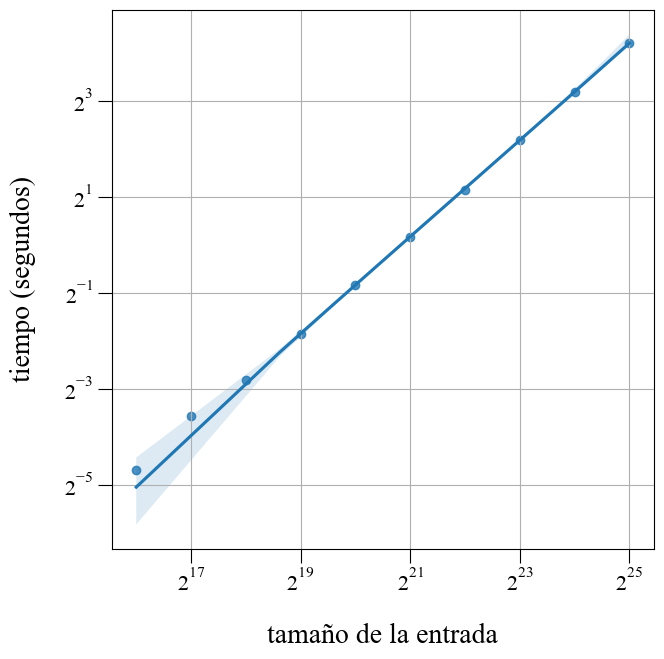
\includegraphics[scale=0.5, clip]{./files/src/.media/aleatorio.png}
    \caption{Tiempo de ejecución del algoritmo de \textit{selección de actividades} en función del tamaño de la entrada, para instancias aleatorias.} \label{aleatorio}
\end{figure}

La relación lineal es bastante clara. Para asegurarnos, calculamos también el coeficiente de Pearson, $\rho$, que mide la correlación lineal entre ambas variables, donde $\rho = 1$ indica una correlación fuerte. El resultado fue $\rho \approx 0.9997$.

% instancias
\subsection{Instancias de interés}

Un análisis del algoritmo indica que lo único que parece alterar el flujo del código\footnote{Notar que, por la cota fija de $2n$ que tomamos para \textit{counting sort}, un rango de intervalos menor a $2n$ no afectará el comportamiento de esta parte del algoritmo. Así también ---por sus características---, el mismo no se verá afectado por el ordenamiento inicial de la entrada.}, en función de la entrada, es 
la cantidad de actividades que son seleccionadas. Donde, por cada actividad seleccionada, se ejecutan dos lineas de código más (en particular, se agrega un elemento más al conjunto de soluciones $P$). %Sin embargo, de implementarse como proponemos, solo agrega un tiempo de ejecución constante, por lo que no debería ser demasiado significativo.
%cada tupla ordenada empieza después (o al mismo tiempo) que cuando termina la última tarea de P. 

Para probar la diferencia de tiempos posibles entre instancias diferentes bajo este criterio ---que tengan cantidades distintas de actividades seleccionables---, realizamos una serie de evaluaciones, siguiendo la metodología de la experimentación anterior, primero con una instancia \textit{comprimida} ---en la que la intersección entre todos los intervalos de las actividades de $A$ es no vacía, por lo que sólo se agrega un elemento al conjunto de soluciones $P$--- y una instancia de entradas \textit{separadas} ---donde la $i$-ésima entrada tiene la forma $(i,\ i+1)$, por lo que se agregan todas las actividades en $A$ al conjunto de soluciones $P$---. 

El siguiente gráfico, nuevamente en escala \textit{log-log} por la naturaleza de las muestra, expone los resultados.

\begin{figure}[!htbp]
    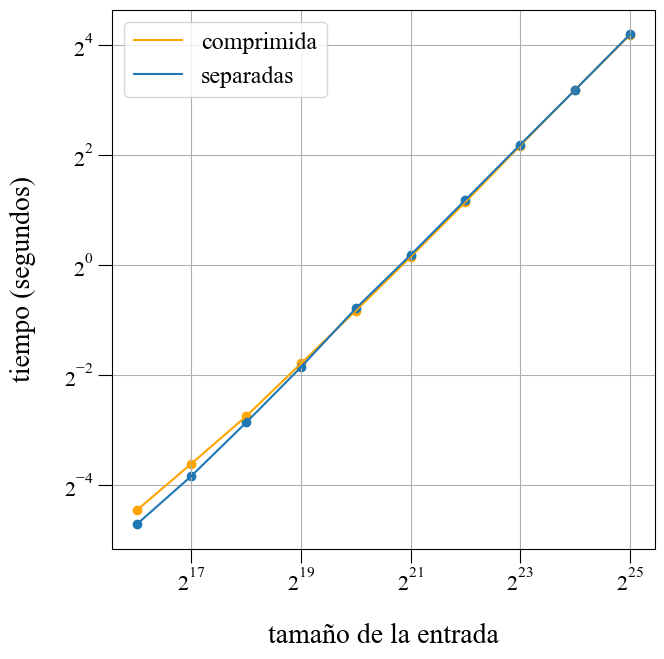
\includegraphics[scale=0.5, clip]{./files/src/.media/comparacion.png}
    \caption{Tiempo de ejecución de la \textit{selección de actividades} en función del tamaño de entrada $n$ y la cantidad máxima $m$ de tareas seleccionables, para \textit{comprimida} ---$m = 1$--- y \textit{separadas} ---$m = n$---.} \label{comparacion}
\end{figure}


Si bien es verdad que, en las entradas más grandes, las instancias de \textit{separdas} parecen haber tomado un poco más de tiempo, la diferencia no resulta significativa. En promedio, \textit{separadas} fue $\approx 20.8$ milisegundos más lenta.
\newpage

% apendice
% \section{Apéndice}
% \input{files/src/apendice.tex}
% \newpage

%bibliografia - requiere que haya citas
% \bibliographystyle{plain}
% \bibliography{./files/citations.bib}
% \newpage

\end{document}
